\documentclass[12pt]{article}
\usepackage{graphicx, color}
\DeclareGraphicsExtensions{.ps,.eps,.pdf} %%%Erlaubte Änderungen
\usepackage{amssymb}
\usepackage{latexsym}
\usepackage{amsmath}
\usepackage{multirow}

\usepackage{listings} % code Darstellung

\lstset{ 			  % code style
	backgroundcolor=\color{white},
	keepspaces=true,
	numbers=left,						% where to put the line-numbers
	numberstyle=\tiny\color{black},
	stepnumber=1,						% the step between two line-numbers
	captionpos=b,						% sets the caption-position to bottom
	tabsize=2,  						% sets default tabsize to 2 spaces
	showstringspaces=false,				        % underline spaces within strings or not
	columns=flexible,
	%breaklines=true					% enter is breakline
	basicstyle={\small\ttfamily},		                % the size of the fonts that are used 
	keywordstyle=\color{blue},
	commentstyle=\color{mygreen},
	stringstyle=\color{red},
	escapeinside={\%*}{*)},
	morekeywords={*,...}
}
\definecolor{mygreen}{rgb}{0,0.6,0}

%\usepackage{enumitem}

\textwidth16cm \textheight23cm
\oddsidemargin0.2cm
\evensidemargin0.5cm
\parindent2ex
\parskip1.5ex plus0.5ex minus0.5ex
\renewcommand{\baselinestretch}{1.37}
\unitlength1.0cm \headheight0cm \topskip-1cm \headsep-1cm
%\pagestyle{empty}

%$\mbox{\boldmath$\mu$}$ for bold greescian letters
%\boldsymbol{\mu} in equations


\newcommand{\bbo}{\mbox{1}\hspace{-3pt}\mbox{I}}
\newcommand{\Na}{\mbox{I}\hspace{-2pt}\mbox{N}}


\newcommand{\real}{\mbox{I}\hspace{-2pt}\mbox{R}}
\newcommand{\indi}{\mbox{1}\hspace{-3pt}\mbox{I}}
\newcommand{\B}{\mbox{I}\hspace{-2pt}\mbox{B}}
\newcommand{\intplus}{\mbox{I}\hspace{-2pt}\mbox{N}}
\newcommand{\integer}{\mbox{Z}\hspace{-4pt}\mbox{Z}}
\newcommand{\F}{\mbox{I}\hspace{-2pt}\mbox{F}}
\newcommand{\var}{\mbox{var\,}}
\newcommand{\cor}{\mbox{cor\,}}
\newcommand{\Var}{\mbox{Var\,}}
\newcommand{\Cov}{\mbox{Cov\,}}
\newcommand{\cov}{\mbox{cov\,}}
\newcommand{\Eur}{\mbox{C\hskip-0.35cm =\,}}


\newcommand{\bbr}{\mbox{I}\hspace{-2pt}\mbox{R}}
\newcommand{\bbn}{\mbox{I}\hspace{-2pt}\mbox{N}}
\newcommand{\bbone}{\mbox{1}\hspace{-3pt}\mbox{I}}
\newcommand{\bbz}{\mbox{Z}\hspace{-4pt}\mbox{Z}}

%

\newtheorem{definition}{Definition}
\newtheorem{theorem}{Theorem}
\newtheorem{corollary}{Corollary}
\newtheorem{proposition}{Proposition}
\newtheorem{lemma}{Lemma}
\newtheorem{remark}{Remark}
\newtheorem{example}{Example}

%  Print review date and 'Draft Version' (From Josullvn, CS, CMU)
\newcommand{\reviewtimetoday}[2]{\special{!userdict begin
/bop-hook{gsave 20 710 translate 45 rotate 0.8 setgray
/Times-Roman findfont 12 scalefont setfont 0 0 moveto (#1) show 0
-12 moveto (#2) show grestore}def end}}
%\reviewtimetoday{\today}{Draft Structure}
% You can turn on or off this  option.

% Bibliography und Erzeugung der bib Datei
\usepackage{array}
\usepackage[backend=bibtex,style=authoryear,maxcitenames=2,giveninits=true,natbib=true]{biblatex}
\renewbibmacro*{volume+number+eid}{%
	\printfield{volume}%
	%  \setunit*{\adddot}% DELETED
	\setunit*{\addnbspace}% NEW (optional); there's also \addnbthinspace
	\printfield{number}%
	\setunit{\addcomma\space}%
	\printfield{eid}}
\DeclareFieldFormat[article]{number}{\mkbibparens{#1}}
\addbibresource{BIB.bib}


\begin{document}
\renewcommand{\thetheorem}{\arabic{theorem}.}
\renewcommand{\theremark}{\arabic{remark}.}
\renewcommand{\thelemma}{\arabic{lemma}.}
\renewcommand{\theproposition}{\arabic{proposition}.}
\renewcommand{\thefootnote}{\fnsymbol{footnote}}


\vspace*{1cm}



\centerline{\LARGE\bf The non-Gaussian exponential SEMIFAR}
\centerline{ \Large\bf and its application as a semiparametric long-memory volatility model }
\vskip.2cm

\vspace{.2cm}

\centerline{\large Yuanhua Feng, Sebastian Letmathe}
\vspace*{-.4cm}
\begin{center}
Faculty of Business Administration and Economics, Paderborn University
\end{center}


%threshold GARCH (TARCH)

\begin{abstract}
\noindent The well-known ESEMIFAR model introduced by \citet{beran2015modelling} simultaneously identifies a deterministic trend as well as short- and long-range dependence. The authors derived statistical properties under the assumption that the stationary part of the ESEMIFAR follows a zero mean FARIMA process with Gaussian innovations. Another finding was that the long-memory parameter could be estimated from the log-transformed process as the Hermite rank of the exponential transformation has rank one. Consequently, the long-memory parameter in the original and the log-transformed process is the same.This paper proposes an extension of the ESEMIFAR to the non-Gaussian case. Under suitable additional assumptions on the distribution of the innovations we show that the Appell rank of the exponential transformation is one as well. Hence, the long-memory parameter is expected to be the same for the original and log-transformed process.Theoretical asymptotic properties of our model are derived. We ensure that data-driven SEMIFAR algorithms are applicable to our proposal. The appropriateness of our approach is then illustrated by the application to financial data. Trend estimation and model selection is implemented with the statistical software R.  



\vskip.2cm

%\noindent{\bf JEL Classification Codes:} C14, C222, G00, G10


\noindent{\bf Key Words:} Long-memory, Exponential SEMIFAR, SEMIFAR algorithms, non-Gaussian, Hermite rank, Appell rank

\end{abstract}
\clearpage
\section{Introduction}

%\section{The Gaussian EFARIMA and ESEMIFAR Model}
%
%\begin{itemize}
%	\item introduction of the Models (see Beran et al., 2015 and Feng \& Zhou, 2015)
%	\item affect of the exponential transformation on the long memory parameter see (Andersen, 1994; Andersen \& Bollerslev, 1997; Robinson, 2001)
%	\item one small application example
%	
%\end{itemize}
%\section{The non Gaussian Case}
%\begin{itemize}
%	\item Introduction of the EFARIMA and ESEMIFAR Model with non-gaussian innovations
%	\item affect of the exponential transformation on the long memory parameter
%	\item Theorem: d does not change for all $X^a, a \in \mathbb{R}_+$ 
%	\item Lemma: Appell rank of tranformations of the form $exp(\lambda X)=Y^\lambda$ is one.
%\end{itemize}
%\section{Appel Rank and Power Rank }
%\begin{itemize}
%	\item calculation of Appell and Power rank for the exponential transformation (assumed to be 1) NACHFRAGEN!!!
%\end{itemize}
%\section{Conclusion/Concluding Remarks}
%\clearpage
\section{Non-Gaussian EFARIMA and ESEMIFAR models}
The following models are formulated to analyse non-negative equidistant financial time series data. Our proposal is particularly designed for cases where the normality assumption would not be suitable, i.e. financial data with heavy tails for example. We follow Beran et. al (2015) and extend the Gaussian EFARIMA and ESEMFIAR by assuming that the innovations follow some other well-known non-Gaussian distribution. To motivate our proposals we first summarize the results under the normality assumption derived by Beran et. al (2015) and illustrate the relationship of the EFARIMA to the EACD$_1$.
\subsection{EFARIMA  and ESEMIFAR models}
We define $X_t$ ($t=1,...N)$ as a nonnegative stationary financial time series. A well-established model for  analysing financial time series data, particularly trade durations,                                                                                                                                                                                                                                                                                                                                                                                                                                                                                                                                                                                                                                                                                                                                                                                          is the multiplicative error model (MEM) which is given by 
\begin{equation}
\label{1}
X_t=\nu \lambda_t \eta_t.
\end{equation}
The scale parameter is denoted by $\nu >0$, $\lambda_t >0$ denotes the conditional mean of $X^*=X_t/\nu$, and $\eta_t$ are i.i.d. random variables. Following Feng and Zhou (2015) we rewrite \eqref{1} as a semiparametric MEM given by
\begin{equation}
\label{2}
X_t=\nu(\tau_t)X^*=\nu(\tau_t)\lambda_t \eta_t,
\end{equation}   
where $\tau_t=t/n$ denotes the rescaled time and where we replaced the scale parameter in \eqref{1} with a nonparametric scale function denoted by $\nu(\tau_t)$. 
By taking the logs we can rewrite \eqref{2} as a semiparametric FARIMA model:
\begin{equation}
Y_t=\mu(\tau_t) + Z_t=\mu(\tau_t)+\xi_t + \epsilon_t,
\end{equation}
where $Y_t=ln(X_t)$, $\mu(\tau_t)=ln[\nu(\tau_t)]$, $Z_t=ln(X^*)$, $\xi_t=ln(\lambda_t)$ and $\epsilon_t=ln(\eta_t)$. Following Beran et. al (2015) we assume that $Z_t$ follows a FARIMA ($p, d, q$) process with zero mean:
\begin{equation}
\label{4}
(1-B)^d\phi(B)(\xi_t + \epsilon_t)=(1-B)^d\phi(B)Z_t =\psi(B)\epsilon_t,
\end{equation}
where $d \in (0,0.5)$ is the long-memory parameter, $\phi(z)=1-\sum_{i=1}^{p}\phi_iz^i$ and  $\psi(z)=1-\sum_{i=1}^{q}\psi_iz^i$ are AR- and MA-polynomials with all roots outside the unit circle. Equation \eqref{4} defines a stationary and invertible FARIMA process with $E(\epsilon_t)=0$ and $var(\epsilon_t)=\sigma^2_{\epsilon}$. Under the strong assumption that $\epsilon_t \sim  N(0,\sigma^2_{\epsilon})$ in $Z_t$ and hence $\eta  \sim   LN(0,\sigma^2_{\epsilon})$ in $X^*_t=exp(Z_t)=exp(\xi_t + \epsilon_t)$, $Z_t$ and $X^*_t$ are explicitly called Gaussian FARIMA and Gaussian EFARIMA respectively.
\subsubsection{Stationary solutions}
 Please note that we do not assume that $\epsilon_t$ is not normally distributed. We extend the results of \citet{beran2015modelling} which were obtained under the log-normal assumption to more general distributions.
 We can write $Z_t$ as a MA($\infty$) process:
\begin{equation}
\label{5}
Z_t=\sum_{i=0}^{\infty}\beta_i\epsilon_{t-i},
\end{equation} 
where $\beta(B)=\frac{\psi(B)}{(1-B)^d\phi(B)}$, and $\beta_i/c_{\beta} i^{d-1}\longrightarrow 1$ for large $i$ with 
\begin{equation}
	c_{\beta}=\frac{|\psi(1)|}{|\phi(1)|} \frac{1}{\Gamma(d)}>0,
\end{equation}
where $\Gamma(\cdot)$ denotes the Gamma-function. Under long range dependence the autocorrelations of $Z_t$ are not summable, since $\rho_Z(k) \approx c^Z_{\rho}|k|^{2d-1}$ with $c^Z_{\rho} > 0$ being a constant. It was shown by Beran (1994), Bondon and Palma (2007), Kokoszka and Taqqu (1995) and Palma (2007) that an FARIMA process has a unique stationary solution given by an infinite moving average representation, for $\phi(B)$ and $\psi(B$ having no common zeros, $\phi(B)$ having roots lying outside the unit circle, and $d\in(-0.5,0.5)$. They further demonstrate, that the MA coefficients in \eqref{5} can then be stated as $\beta_i=\psi(1)i^{d -1}(\phi(1)\Gamma(d))^{-1}+O(i^{-1})$ as $i\rightarrow \infty$. 
%Note that \eqref{5} represents a stationary solution of the FARIMA process given by \eqref{4}.
Let $\beta_{max} = sup(\beta_i)$ and $\beta_{min} = inf(\beta_i)$. Feng and Zhou (2015) derived the following conditions for the existence of a stationary solution of $X^*$:

\textbf{A1:} $Z_t$ is a stationary and invertible FARIMA process given by \eqref{4}

\textbf{A2:} The second order moments $E(\eta_t^{2u\beta_{max}})$ and $E(\eta_t^{2u\beta_{min}})$ exist, where $u$ is some positive number.
Condition A2 is sufficient for the existence of all the terms in \eqref{7} and A1 indicates that in \eqref{5} $\sum_{i=0}^{\infty}\beta_i<\infty$ and $E(\epsilon_t)=0$. If both conditions hold $X^*_t$ converges and hence 
Lemma 1 in Feng and Zhou (2015) implies with regard to A1 and A2 that the stationary solution for $X^*_t$ is given by:
\begin{equation}
\label{7}
	X^*=\prod_{i=0}^{\infty}\eta^{\beta_i}_{t-1}.
\end{equation}
Moreover, the authors indicated that condition A2 is not affected by $d$ and jointly depends on the marginal distribution of $X^*$, the value of $u$, and $\beta_i$. For log-normal innovations A2 is always fulfilled.


Hier noch weiter (stationary solutions)


\subsection{Long memory properties}
In the case of Gaussian innovations \citet{beran2015modelling} derived precise formulas for moments, autocovariances and autocorrelations as well as long-memory properties. The authors indicated that the long-memory parameter is the same in the original process $X_t$ and the transformed process $Y_t$ ($Z_t$). \citet{menendez2013trend} indicated that every monotonous transformation has Hermite rank one. Consequently, it holds that $X_t=G(Z_t) =\nu(\tau_t) X^*_t=\exp(Y_t)=\exp(\mu(\tau_t)+Z_t)$ has Hermite rank one as well. The expansion of transformed RVs by means of orthogonal polynomials is possible only for a very limited amount of distribution classes, e.g., normal and exponential distribution \citep{beran2013limit}.  Therefore, in the face of non-Gaussian innovations it is not possible to represent $G(Z_t)$ in terms of a Hermite expansion. However, if the underlying transformation function fulfils  certain conditions and under suitable assumptions on the marginal distribution of $Z_t$, it is feasible to write the transformation function by means of an Appell polynomial expansion which can be considered to be a generalization of Hermite polynomials \citep{schutzner2009asymptotic}.

FIXME
%

%\subsubsection{Appell rank}
% The explicit formal definition of Appell polynomials strongly depends on the moment generating function of the linear process (see Beran et. al 2013) as the so called generating function of Appell polynomials is given by
%
%\begin{equation}
%M_Z(x, z)=\frac{exp(xz)}{m_{Z}(z)}=\sum_{i=0}^{\infty}\frac{z^i}{i!}A_i(x),
%\end{equation} 
%where $A_i(x)$ are polynomials of degree $i \in \mathbb{N}$, $z \in \mathbb{R}$ and $m_{Z}=exp(zZ_t)$ denotes the moment generating function of $Z_t$. Please note that 
%\begin{equation*}
%	A_i(x)=\frac{d^i}{dz^i}[M_Z(x, z)]_{z=0}.
%\end{equation*} 
%
%The set-up of an infinite-order Appell expansion requires complex and strong assumptions on both the expansion function itself and the underlying distribution. Because it turns out that the criterion of an infinitely differentiable (analytic) expansion function is not sufficient for an Appell polynomial representation, the authors refer to a smaller functional sub-class here. In particular, they consider entire functions of a certain exponential order type (Beran et al., 2013, [Definition 3.9]). According to Beran et al. (2013, [Theorem 3.4]) the following conditions have to hold: 
%  
%  \textbf{A3:} $G$ is supposed to be an entire function with exponential order type $\tau$, where $\tau$ is a finite positive number. Such a class of functions is defined by $C(\tau_1/2)$ hereinafter.
%  
% \textbf{A4:} The moment generating function of $Z_t$, which is given by  $m_{Z_t}(s)=E(e^{s \beta \epsilon})=E(\eta^{s \beta})$,
% has to be finite in an open neighbourhood around $U_{\tau}=\{-s < \tau < s\}$. Note that this condition implies that all absolute moments, given by $E[|Z_t|^n]$, are finite (Beran et al., 2013).
%% $|G(\cdot)|=|e^x|\leq e^{\tau x}$ 
%
%\begin{lemma}
%	Assume that $Z_t=ln(X^*_t)$ is an invertible and stationary FARIMA(p,d,q) process with zero mean as defined in \eqref{4}. If conditions A3 and A4 hold the general Appell rank of $G(Z_t)=\exp[a(\mu(\tau_t)+Z_t)]
%	=[\nu(\tau_t)(X^*_t)]^a=X_t^a$, with $a>0$ is one.
%\end{lemma}
%As $\lim\limits_{x \rightarrow \infty}{\frac{G(x)}{exp(\tau x)}}=\frac{exp(x)}{exp(\tau x)}=0$ for $\tau >1$, it is obvious that  $G \in C(\tau_1/2)$  for $\tau_1 \geq 2$ with $\tau_1 < \tau$. Consequently $m_{Z_t}(z)$ has to be defined in $U_\tau=\{|z|<2+\delta\}$, with $\delta \rightarrow 0$. Condition A4 with respect to $G$ is fulfilled by:
%\begin{example}
%	The log-normal inverse gaussian innovations $\eta_t$ with $\epsilon_t \sim $NIG(0, $\omega$, $\alpha$, $\beta$)
%\end{example}
% \begin{example}
% 	The log-variance gamma innovations $\eta_t$ with $\epsilon_t \sim $VG($0$, $\alpha$, $\beta$, $\lambda)$
% \end{example}
%\begin{example}
%The log-skewed normal innovations $\eta_t$ with $\epsilon_t \sim $SN($0$, $\omega$, $\alpha)$
%\end{example}
%
%
%
%%Examples reinhaun mit log-sas, box-cox normal, Birnbaum saunders (power rank noch indizieren)!!!!!!!!!!!!!
%% Beispiele (Verteilungen) nehmen bei denen die mgf überall definiert ist. Dann fällt der Beweis und die Definiton der Klasse weg.
%% Danach Powerrank indizieren. Einfach und besser anwendbar.
%% Kovarianzfunktion usw. vom Originalprozess mit transformiertem Prozess vergleichen.
%% Als nächste Power rank lesen ung weiteres Kapitel mit Power rank
% 
%% Suitable distributions:
%% \begin{itemize}
%% \item skewed normal 
%% \item variance gamma
%% \item normal inverse gaussian
%% \item bilateral gamma
%% \end{itemize}
%
% 
%   
% 
%%\begin{example}
%%	We assume that $X^*$ is a log-Laplace process with log-Laplace distributed $\eta_t$ with $\epsilon_t \sim La(0,\sigma)$. Then we have the moment generating function $m_{X^*}(s)=e^{\mu z}(1-\sigma^2 z^2)$. By inserting the corresponding parameters $\mu=0$ and $\sigma>0$ we have $\frac{1}{1-\sigma^2 z^2}$ and subsequently 
%%	\begin{align*}
%%		M_{X^*}(x,z)=&e^{xz} (1-\sigma^2 z^2)=\sum_{n=0}^{\infty}\frac{x^n z^n}{n!}- \sum_{n=2}^{\infty}\frac{x^{n-2} z^{n}\sigma^2}{n!}\\
%%		=&1+xz + \sum_{n=2}^{\infty}\frac{z^n}{n!}(x-(n^2-n)\sigma^2)x^{n-2}
%%	%	=& 1-\sigma^2 z^2 +\sum_{n=1}^{\infty}\frac{s^n}{n!}(1-\sigma^2 s^2)x^n,\\                                                                                                    
%%	\end{align*}
%%	so that
%%	\begin{align*}
%%		A_0^{La}&=1,\quad A_1^{La}=x + 1,\\    			%\quad A_2^{La}=x^2-2\sigma^2,\\
%%A_n^{La}&=(x^2-(n^2-n)\sigma^2)x^{n-2}.
%%	\end{align*}
%%%	\begin{equation}
%%%		A_n^{La}=(x^2-(n^2-n)\sigma^2)x^{n-2}		%A_n^{La}=(x^2-(n+2)(n+1)\sigma^2)x^{n-2} \qquad \qquad \qquad (n\geq2). 
%%%	\end{equation}
%%\end{example} 
%
%%\begin{example}
%%We assume that $X^*$ is a log-normal-inverse Gaussian (NIG) process	with log-NIG innovations $\eta_t$ with $\epsilon_t \sim NIG(\mu, \alpha,\beta, \delta)$. Then the moment generating function is given by $m_{X^*}(z)=exp(\mu z+\delta(\gamma - \sqrt{\alpha^2-(\beta+z)^2}))$. By inserting the corresponding parameters $\mu=0$, $\alpha\rightarrow \infty$, $\beta = 0$ and $\delta \in \real$ we have $exp(\delta(-\sqrt{\alpha^2-z^2}))$ and subsequently
%%
%%
%%%$\exp(\delta(\gamma - \sqrt{\alpha^2-(\beta+z)^2}))$ and subsequently
%%\begin{align*}
%%M_{X^*}(x,z)=e^{xz} e^{\delta(\alpha-\sqrt{\alpha^2-z^2})}=\sum_{n=0}^{\infty}\frac{x^nz^n}{n!} \sum_{n=0}^{\infty}\frac{\delta^n (\alpha-\sqrt{\alpha^2-z^2})^n}{n!}
%%\end{align*}
%%NACHFRAGEN!!!!!!!!
%%\end {example} 
%
% If conditions A3 and A4 both hold Theorem 3.4 in Beran et al. (2013) is applicable and a relatively simple expression to calculate the $j_{th}$ Appell coefficient is given by  
%	\begin{equation}
%	\label{9}
%		a_{app,j}=E[G^{(j)}(Z_t)].
%	\end{equation}
%	Analogue to the Gaussian case the Appell rank is defined as the smallest integer j $\geq 1$ such that
%		\begin{equation}
%	\label{10}
%	a_{app,j}=E[G^{(j)}(Z_t)] \neq 0.
%	\end{equation}	
%
%
%\textbf{noch bearbeiten}
%If $E(|Z_t|^n)<\infty, n \in \mathbb{N}$ holds, then all Appell polynomials up to order $n$ exist and we can define a finite-order expansion for $n\geq1$ given by
%\begin{equation}
%	G(Z_t)-E(G(Z-t))=\sum_{i=1}^{n}\frac{a_{app,i}}{i!}A_i(Z_t)+R_n(Z_t),
%\end{equation}
%where $R_n$ is a remainder term (Giraitis et al., 2012).
%Similar to the Gaussian case and the corresponding role of the Hermite rank, the Appell rank is of central importance for deriving limit behavior of subordinated processes with linear underlying. Furthermore, the convergence of sums of Appell polynomials is a crucial indicator for LRD patterns in the linear process. For functions $G$ enabling a valid infinite-order expansion and therefore satisfying the analyticity conditions A3, the limit distribution of \eqref{5} is basically the same as in the Gaussian case. This finding is mainly founded on the examinations of Avram and Taqqu (1987), Giraitis (1985), Giraitis and Surgailis (1989) and Surgailis (1982). Surgailis (1982) was the first studying the (non-central) limiting behavior of sums of polynomials of linear processes under the stringent requirements on the expansion function discussed above. Here, investigations are performed using another related rank notion, often called exponent rank in the literature. Based on these results, Avram and Taqqu (1987) present the calculation of Appell polynomials for stationary linear moving average processes with i.i.d. innovations and slowly decaying coefficients. While for $j_{app}>𝑏1/(1-2d)$ the usual central limit theorem holds (Sch{\"u}tzner, 2009, pp.15-16) and the limit is Brownian motion, they show, that under the condition $E[\epsilon_t^{2j_{app}}]<\infty$ and $j_{app}<1/(1-2d)$, the convergent distribution of partial sums can be expressed in terms of the Hermite process depending on the Appell rank, $j_{app}$. The latter includes a slower rate of convergence. The non-central limit can be given by the same Wiener-Itô integral, as in the Gaussian case. The leading term in the expansion is given by $(a_{app}/j_{app}!)A_{j_{app}}(Z_t)$
%and determines the asymptotic properties of the partial sum process (reduction principle). Surgailis and Vaičiulis (1999) generalize these results by assuming the innovations in \eqref{5} to be a sequence of martingale differences. Surgailis (2000) studies nonlinear functions of processes that are the sum of a moving average process and a nonlinear weakly dependent sequence. He shows that the limit distribution of partial sums of these processes is still determined by the Appell rank. Thus, we have an invariance against additive noise. In Beran and Schützner (2008), the Appell expansion of a multiplicative volatility process is considered. In particular, this process is the product of an i.i.d. RV and a stationary nonlinear series with long memory. It turns out, that the symmetry of the RV is crucial for the limiting behavior of partial sums. 
%\subsubsection{Power rank}
% 
%The Hermite expansion is only valid for Gaussian processes, and the Appell expansion is very restricted due to the stringent requirements on the expansion function and the underlying distribution. Moreover it is rather difficult to obtain asymptotic expressions for autocovariances and autocorrelations. Another approach which circumvents traditional polynomial expansion is the decomposition approach introduced by Ho and Hsing (1996, 1997) (see also Hsing (2000) and Koul and Surgailis (2002) for an exposition).  The method avoids the procedure of traditional polynomial expansion and so does not impose such strict regularity conditions on the expansion function. In Ho and Hsing (1996) empirical (long memory) moving average processes are formally approximated by an expansion consisting of a finite amount of uncorrelated terms. It is shown, that this amount is related to the size of the memory parameter 𝛿. Limit theorems for functionals of moving average processes are derived in Ho and Hsing (1997). Here it is proposed that depending on the decay of the coefficients in the MA representation, it is possible to decompose the partial sums of the transformation into two (asymptotically) uncorrelated elements.The authors show that for long memory in the underlying, these elements converge to a central and non-central limit, respectively (Ho and Hsing, 1997, p.1636). Moreover, the NCLT depends on the so-called power rank. Hsing (1999) investigates asymptotic distributions of partial sums, where the transformation is a bounded and measurable function and the innovations in \eqref{5} satisfy a standard symmetric $\alpha$-stable distribution. It is shown that the convergence of the partial sums depends again on the speed of decay of the moving average coefficients. The non-central limit depends on the so-called power rank.
%
%%4.2.2.1 The Conceptual Idea of Decomposition and the Role of the Power Rank
%To give an impression of the method according to Ho and Hsing (1996, 1997), we define 
%\begin{equation}
%Y_{n,0}=n
%\end{equation}
%and
%\begin{equation}
%\label{13}
% Y_{n,r}=\sum{t=1}^{n}\sum_{1\leq i_1<\cdots<i_r<\infty}^{}\prod_{s=1}^{r}a_{i_s}\epsilon_{t-i_s}
%\end{equation} 
%where $i_1<i_2<\cdots<i_r$ and $r\leq 1$ are positive integers (Ho and Hsing, 1996, p.994). In case the coefficients in \eqref{5} decay like $a_i\sim c_ak^{d-1}$ as $i\rightarrow\infty$, where $c_a>0$ and $d\in(0,0.5)$, it can be shown, that for $r\delta=r(1-2d)<1$ the process given by $\sum_{1\leq i_1<\cdots<i_r<\infty}^{}\prod_{s=1}^{r}a_{i_s}\epsilon_{t-i_s}$ in \eqref{13} exhibits long memory (Ho and Hsing, 1997, p. 1638). Then, for different $r$, $Y_{n,r}$ are uncorrelated. Let us, following Ho and Hsing (1996), rewrite the expression $r\delta<1$ to $r<1/\delta$ and define $p^*=\lfloor1/\delta\rfloor$, as the integer part of $1/\delta$. Consequently, for $1\leq r\leq p^*$, each $Y_{n,r}$ is decomposed into long memory terms. Otherwise, for each $r>p^*$, all summands in \eqref{13} have short memory.
%Now define, 
%\begin{equation}
%\label{14}
%G_{\infty}(z)=E[G(z+Z_t)],
%\end{equation}
%where $z\in \mathbb{R}$ and $G$ is a measurable function. \eqref{14} is assumed to be $p*$ times differentiable at $z=0$. The (centered) partial sum is given by 
%\begin{equation}
%\label{15}
%S_n=\sum_{t=1}^{n}[G(Z_t)-E[G(Z_t)]]=L_{n,p^*}+S_{n,p^*},
%\end{equation}
%with 
%\begin{equation}
%\label{16}
%L_{n,p^*}=\sum_{r=1}^{p^*}G_{\infty}^{(r)}(0)Y_{n,r}
%\end{equation}
%and 
%\begin{equation}
%\label{17}
%	S_{n,p^*}=\sum_{t=1}^{n}[G(Z_t)-E[G(Z_t)]]-L_{n,p^*}
%\end{equation}
%where $G_{\infty}^{(r)}(0)=\frac{d^r}{dz^r}E[G(z+Z_t)]|_{z=0}$ is the 𝑟th derivative of $G_{\infty}(0)$ (Hsing, 2000, p. 21). Note, that for $r\delta=r(1-2d)<1$, $S_{n,p^*}$ and $Y_{n,r}$ are asymptotically uncorrelated (Ho and Hsing, 1997, p.1641).
%
%
% Following Ho and Hsing (1997) the power rank $b$ is defined as the lowest integer $r\ge 1$ such that $G_{\infty}^{(r)}(0)\neq0$. For all $1\leq r < b$ we have $ G_{\infty}^{(r)}(0)=0$. Alternatively, we can write
% \begin{equation}
% 	b=inf\{r\geq 1,G_{\infty}^{(r)}(0)\neq 0\},
% \end{equation}
% where $G_{\infty}(x)=E[G(x+X)]$.
%The corresponding rank coefficient is given by $G_{\infty}^{(r)}(0)$. It can be shown, e.g., for transformation functions $G(x)=x^2,\quad x^3,\quad x^4,\quad x^3-3x,\quad x^4-6x^2,\quad sin(x)$ and $exp(x)$ the corresponding power ranks are 2, 1, 2, 3, 4, 1 and 1, respectively (Sang \& Sang, 2016, p.7).
%
%$L_{n,p^*}$ and $S_{s,p^*}$ are the (asymptotically uncorrelated) long memory and short memory component of \eqref{15}, respectively.
%Thus, we can formulate the main message in Ho and Hsing (1997), which is that the partial sum has a decomposition of the form 
%\begin{equation}
%	S_n=\text{noncentral part} + \text{central part}
%\end{equation}
%(Ho and Hsing, 1997). Now, if $L_{n,p^*}\neq 0$ the convergent behavior of $S-n$ is determined by the leading term in the expansion of $L_{n,p^*}$, which is $G_{\infty}^{(b)}Y_{n,b}$ (Lévy-Leduc and Taqqu, 2013). Only if there is no non-central part in the decomposition, thus $L_{n,p^*}=0$, the short memory component dominates and the limit distribution follows a central ($\sqrt{n}$ rate) limit theorem. If $E[G^2(Z_1)<\infty$, $E[\epsilon_1^{2bV8}<\infty$, where $2bV=max\{2𝑏,8\}$, and another (technical) regularity condition (Ho and Hsing, 1997, p.1639) is satisfied, then for $b\leq p^*$, implying the presence of a noncentral component, one gets a Hermite process of rank $b$ as distributional limit. This means that the limit can be stated as $G_{\infty}^{(b)}(0)$ times a random variable, expressible by the Wiener-Itô integral. In the case $b>p^*$ the limit of the $\sqrt{n}$-standardized partial sum is Brownian motion. Note that the central limit is derived under slightly differing conditions on the innovation process. Hsing (2000) draws the conclusion, that the applied assumptions to obtain the CLT and NCLT are not the weakest possible. Corresponding reductions are proposed, e.g., in Giriaitis and Surgailis (1999) and Wu (2006).
%The parallels to the Gaussian case are already indicated here. For a standard normal process the Hermite rank and power rank coincide. This is proved by Bai and Taqqu (2016a) under the application of the theory of the generalized Weierstrass transformation. For this, the authors assume $G_{\infty}(z)$ to be analytic on $z\in(-\sigma,+\sigma)$, for some $\sigma>0$. The expansion of $G_{\infty}(z)$ can then be written as 
%\begin{equation}
%G_{\infty}(z)=\sum_{s=0}^{\infty}\frac{G_\infty^{(s)}(0)}{s!}z^s
%\end{equation}
% (Bai and Taqqu, 2016a, p.3).
%At this point, we would also like to emphasize the close relation to the Appell polynomial expansion. Therefore, consider again $G_{\infty}^{(r)}(0)$ in \eqref{15}, \eqref{16} and \eqref{17}. Having a closer look at the decomposition \eqref{13}, we can see $G_{\infty}^{(r)}(0)$ and $a_{app,j}=E[G^{(j)}(Z_t)]$ play similar roles. The short-memory part $S_{n,p^*}$ can be interpreted as a remainder term, which is stressed in \eqref{17}, and is therefore related to $R_n(Z_t)$ in \eqref{11}. The main difference is the requirement of the original $G$ being a smooth function in the Appell context, whereas the Ho and Hsing approach typically includes a smooth function $G_{\infty}$. We follow Ho and Yang (2007) and formulate a simplified version of the technical conditions introduced by Ho and Sing (1997).  If the $r_{th}$ derivative $G^{(r)}$ of $G_{\infty}^{(r)}$ exists we define
%\begin{equation}
%	G^{(r)}_{j,\lambda}(x)=\sup_{|y|\leq\lambda}|G_j^{(r)}(x+y)|, \qquad \lambda \geq 0.
%\end{equation} 
% Let $r \in \mathbb{N}$ and $\lambda \geq 0$. Then it has to hold that
% 
%\textbf{A5}: $G^{(r)}(z)$ exists for all $z$ and $G^{(r)}$ is continuous;
%
%\textbf{A6}: For all $z \in \mathbb{R}$,	
%\begin{equation}
% \sup_{I\subset \{1,2,\cdots\}}E[G^{(r)}_{\lambda}(z+\sum_{i\in I}^{}a_i\epsilon_i)]^4<\infty,
%	\end{equation}
%	where the sup is taken over all subsets.
%	\begin{lemma}
%		Assume that $Z_t=ln(X^*_t)$ is an invertible and stationary FARIMA(p,d,q) process with zero mean as defined in \eqref{4}. If conditions A5 and A6 hold the general power rank of $G(Z_t)=\exp[a(\mu(\tau_t)+Z_t)]=[\nu(\tau_t)(X^*_t)]^a=X_t^a$, with $a>0$ is one.
%	\end{lemma}
%In a recent paper, by applying the decomposition method of Ho and Hsing (1996, 1997), Sang and Sang (2016) investigate the memory properties of transformations $G(Z_t)$ with $E[G^2(Z_t)]<\infty$. Considering special expansion functions, their findings are applicable to  FARIMA($p,d,q$) processes that are not necessarily Gaussian. Under a “quite mild” smoothness condition on $G_{t-1}$ (Wu, 2006, p.4), it is shown, for $b(1-2d)<1$, where $d\in(0,0.5)$, the transformation $G(Z_t)$ has long memory, while for $b(1-2d)>1$ it exhibits short memory (Sang and Sang, 2016, p.5). For FARIMA($p,d,q$) models the named long memory condition can be extended by including $b(1-2d)=1$.
%Following the basic intuition of Dittmann and Granger (2002), an explicit formula for relating memory properties of a  FARIMA and the persistence in its nonlinear transformation is provided. The subordinates’ memory is shown to depend not only on its underlying but also on the size of the power rank, $b$. Under the same condition as above, the transformation $G(Z_t)$, where $Z_t$ is a stationary FARIMA($p,d,q$) with differencing in a range $0<d<0.5$, is a long memory process, $LM(\tilde{d})$, with
%\begin{equation}
%\label{23}
%	\tilde{d}=(d-0.5)b+0.5,
%\end{equation}  for $b(1-2d)<1$. In the opposite case, it is a short memory process, $LM(0)$, for $b(1-2d)>1$ but $(b-1)(1-2d)<1$ (Sang and Sang, [Theorem 2.2]). Again (comparable to the Gaussian case) for a transformation of rank $b=1$ the long memory parameters of transformed and re-transformed process are approximately equal. It can further be concluded that a long memory transformation can never result from a short memory series $Z_t$, because the transformation cannot increase the resulting process’ memory. In general, if $Z_t$ is a short memory process with absolute summable coefficients, under another smoothness condition (Wu, 2006, pp.4-5) which resembles the conditions A5 and A6, the transformation $G(Z_t)$ also exhibits short memory irrespective of the transformation function. This means that the power rank does not play a role in this set-up. Similar to the results in the Hermite expansion context, antipersistence is demonstrated to be a more fragile property than positive memory. Sang and Sang (2016) show this, by applying the square transformation to a FARIMA($0,d,0$) with negative memory $−1<d<0$. The post-transformed process is proposed to be $LM(0)$, i.e., the property of antipersistence has vanished (Sang and Sang, 2016, p.6).
%
%Unfortunately, only an indication of long-range dependent structures in the linear process %underlying
%can be given by the convergence of the partial sums of Appell polynomials. However, to our knowledge, there is no opportunity to draw inference from the memory size of a non-Gaussian linear process on the exact strength in persistence of its non-linear transformation to date. This is essentially due to the distributional specificity of Appell polynomials. So far, explicit findings of the form discussed above have only been provided in the context of Gaussian subordination by the usage of Hermite polynomials (Dittmann and Granger, 2002). Therefore, Sang and Sang (2016) assume a pioneering role in bridging the gap between exact memory characteristics of an (original) stationary linear underlying process and its nonlinear subordinated sequence. To verify their results the authors did a simulation study where they investigated the behaviour of the long memory parameter for some common transformation functions. In contrast to Dittman and Granger (2002) they 
%
%Based on these results we formulate the following Theorem with regard to the effect of the transformation $G$ on the long memory parameter $d$.
%\begin{theorem}
%	Under the assumptions that $Z_t=ln(X^*_t)$ is an invertibel and stationary FARIMA(p,d,q) process with zero mean as defined in \eqref{4} and that Lemma 1 or Lemma 2 hold, the long memory parameter of the transformed process $Y_t$ or $Z_t$ and the re-transformed process $X_t$ or $X^*_t$, remains the same. 
%\end{theorem}
%
%\section{Extensions}
%In this section we concentrate on the properties of the EFARIMA and ESEMIFAR model and its relation to the well known class of exponential GARCH-type models. In particular the FIEGARCH process (fractionally integrated exponential GARCH) introduced by Bollerslev and Mikkelsen (1996) which is a long-memory extension of the EGARCH model proposed by Nelson (1991). It is already proved by Lopes and Prass (2012) that under relatively less restrictive conditions
%a FIEGARCH(p, d, q) process can be formulated as a FARIMA(p, d, 0) process. Consequently, a semiparametric extension of a FIEGARCH model after introducing a scale function could be rewritten as an ESEMIFAR model. Moreover, asymptotic formulas for the autocovariances and autocorrelations of $X^*$ t are presented.








\subsection{The SEMI-LM-GARCH model}
The autoregressive conditional heteroscedasticity (ARCH) model proposed by \citet{engle1982autoregressive} and its generalisation, the generalized ARCH (GARCH)) model, introduced by \citet{bollerslev1986generalized} , is a well-known volatility process approach for modelling non-constant conditional variances. This is of major interest especially for  fitting financial time-series and their frequently observed characteristic of conditional heteroscedasticity and volatility clustering \citep{mandelbrot1963new}. Following  \citet{baillie1996fractionally} a common representation of a GARCH(p,q) model is given by
\begin{align}
	\epsilon_t^2&=e^2_th_t\iff\epsilon_t=e_t\sqrt{h_t}, \\
	h_t&=\alpha_0+\sum_{i=0}^{q}\alpha_i\epsilon_{t-i}+\sum_{j=1}^{p}\beta_jh_j=\alpha_0+\alpha(B)\epsilon_t^2+\beta(B)h_t
\end{align}
where $e_t$ being an i.i.d. standard normal random variable, the square root of $h_t$ denotes the conditional standard deviation, $\alpha_0>0$ and $\alpha_1,\dots,\alpha_q,\beta_1\dots\beta_p\geq0$. $\alpha(B)=\sum_{i=1}^{q}\alpha_iB^i$ and $\beta(B)=\sum_{j=1}^{p}\beta_jB^j$. The GARCH process can also be given by an ARMA(max(p,q)q) type representation in $\epsilon_t^2$ of the form
\begin{equation}
\label{10}
(1-\alpha(B)-\beta(B))\epsilon^2_t=\alpha_0+(1-\beta(B))u_t,	
\end{equation}
where $u_t=\epsilon^2_t-h_t$ is a zero-mean process describing the innovations in the conditional variances. See also \citet{feng2008modelling} for an extension of this model to high-frequency financial data. In the context of this paper, we are particularly interested in the long memory structures to arise in the ACF of absolute and squared market returns (see \cite{ding1993long}). Following \citet{baillie1996fractionally} a fractionally integrated GARCH (FIGARCH) may be written as
\begin{equation}
\label{14}
\tilde{\phi}(B)(1-B)^{\tilde{d}}\epsilon_t^2=\alpha_0+[1-\beta(B)]u_t,
\end{equation}
where $\tilde{\phi}(B)\equiv (1-\alpha(B)-\beta(B))(1-B)^{-1}$ with all roots of $\tilde{\phi}(B)$ and $[1-\beta(B)]$ outside the unit circle and $0<\tilde{d}<1$. By rearranign the terms in \eqref{14} The conditional volatility $h_t$ is now given by
\begin{equation}
	h_t=\alpha_0[1-\beta(1)]^{-1}+\{1-[1-\beta(B)]^{-1}\tilde{\phi}(B)(1-B)^{\tilde{d}}\}\epsilon^2_t.
\end{equation}
Note that the FIGARCH is not second order stationary because it exhibits an infinite unconditional variance. 
A model closely related to the FIGARCH model is the LM-GARCH Model which belongs to the framework of conditionally heteroscedastic processes introduced by \citet{robinson1991testing}. Following \citet{karanasos2004autocorrelation} (cf. Robinson 2001)FIXME  we define the LMGARCH(p, d, q) model as 
\begin{equation}
\label{15}
\tilde{\phi}(B)(1-B)^{\tilde{d}}(\epsilon_t^2-\alpha_0)=[1-\beta(B)]u_t.
\end{equation}
Here the authors model the squared residuals accounting for the deviations from $\alpha_0 \in \mathbb{R}_+$. This centralisation enables us to analogously define the LMGARCH to the FARIMA model for the mean \citep{conrad2006garch}. According to (23) and \eqref{15} we have $E(\epsilon_t)=0$, $\Cov(\epsilon_t,\epsilon_{t-i})=0$ for $i\geq1$ and the unconditional variance with $E(\epsilon^2_t)=\alpha_0<\infty$. Moreover, based on the exponential GARCH (EGARCH) proposed by Nelson (1991), Bailie and Mikkelsen (1996a)FIXME introduced the fractionally integrated exponential GARCH (FIEGARCH) where the logarithm of the conditional variance is modelled as a fractionally integrated process. The EGARCH and FIEGARCH accounts for the so-called leverage effect which usually has short-term effects on the dependence structure of the underlying process. Additionally, no constraints on the parameters are needed as the conditional variance is positive by definition. Following \citet{nelson1991conditional} the EGARCH can be parameterized as an ARMA (p,q)
\begin{equation}
	\log(h_t)=\alpha_0+\tilde{\phi}(B)^{-1}(1+\psi(B))g(e_{t-1}),FIXME
\end{equation}
where $\psi(B)=1+\sum_{i=1}^{q}\psi_iB^i$ are the MA coefficients and $\phi(B)$ and $\psi(B)$ have no common roots. $g(e_{t})=\Theta_{e_t}+\gamma[(|e_t|-E|e_t|)]$ is the news impact function and $\Theta$, $\gamma$ $\in \mathbb{R}$. As already indicated by Nelson (1991) the EGARCH can be extended for fractional orders of integration. Following \citet{bollerslev1996modeling} the extension to the FIEGARCH is given by  
\begin{equation}
\log(h_t)=\alpha_0+\tilde{\phi}(B)^{-1}(1-B)^{-d}[1+\psi(B)]g(e_{t-1}).FIXME
\end{equation}
However, for practical purposes we use the following definition for the FIEGARCH
\begin{equation}
\label{16}
\tilde{\phi}(B)(1-B)^{d}\log(h_t)=\alpha_0+\sum_{i=1}^{p}(\alpha_j|e_{t-i}|+\gamma_ie_{t-i}),
\end{equation}
where $\gamma_i \neq 0$ controls for the existence of leverage effects. Please note that there are various slightly different definitions of a FIEGARCH process. Definition \eqref{16} is also considered in the software S-Plus. It can be shown that, under certain mild conditions, these definitions are equivalent to each other \citep{lopes2012theoretical}. Moreover, the FIEGARCH nests the integrated EGARCH (IEGARCH) and the EGARCH  $d=1$ and $d=0$ respectively. With regard to the FARIMA, ${\log(h_t)}$ is second-order stationary and invertible for $d\in\{-0.5;0.5\}$, see, e.g. \citet{hosking1981fractional}. Another type of GARCH-type model is the so called Log-GARCH model which was independently introduced by Geweke (1986), Pantula (1986) and Milhoj (1987). The Log-GARCH model is given by
\begin{equation}
\label{17a}
	\log(h_t)=\alpha_0+\sum_{i=1}^{p}\alpha_i\log(\epsilon_{t-i}^2)+\sum_{j=1}^{q}\beta_j \log (h_{t-j}).
\end{equation}
Pantula (1986) among others showed that \eqref{17a} admits an ARMA-type representation. Analogously to \eqref{10} we can rearrange the terms in \eqref{17a} and it follows that
\begin{equation}
[1-\alpha(B)-\beta(B)]log(\epsilon_t)=\alpha_0+[1-\beta(B)][\log(\epsilon_t^2)-\log(h_t)].	
\end{equation}  
In correspondence to \eqref{14} we then have
\begin{equation}
\label{19a}
\tilde{\phi}(B)(1-B)^d log(\epsilon_t)=\alpha_0+[1-\beta(B)]\tilde{u},	
\end{equation}
where $\tilde{u}=[\log(\epsilon_t^2)-\log(h_t)]$. \eqref{19a} is called a long-memory Log-GARCH (LM-Log-GARCH) model.
%\begin{equation}
%	\label{18a}
%\log(\epsilon_t^2)=\omega^* + \phi(B) \log(\epsilon_{t-i})-\beta(B)\tilde{\xi)_{t-1}}+\tilde{\xi_t},
%\end{equation}  
%where $\tilde{\xi_t}=\log (e^2)-E[\log (e^2)]$ and $w^*= \alpha_0 + E[\log (e^2)](1-\sum_{j=1}^{q}\beta_j)$. Factorizing with $(1-B)^d$ yields

\subsubsection{Semiparametric estimation}
 Let $x_t$ denote the stock prices of some stock index and $r_t$ their corresponding (log-) returns. Consider the equidistant time series model
\begin{equation}
\label{17}
	r_t=\mu +\sigma(\tau)\epsilon_t
\end{equation}
where $\mu$ is an unknown constant, $\sigma(\tau)$ a smooth scale function and $\epsilon_t^2$ is assumed to follow a long-memory GARCH process, i.e. a FIGARCH, FIEGARCH or LM-GARCH process defined by \eqref{14}, \eqref{15}and (28). We assume that there are strictly stationary solutions for all these long-memory GARCH processes such that $E(\epsilon_t^8)<\infty$. This assumption is needed for the nonparametric estimation of $\sigma(\tau)$ \citep{feng2004simultaneously}. Moreover, it is assumed that $var(\epsilon_t)=E(\epsilon_t^2)=1$.
%\begin{equation}
%	r_t=\mu(\tau)+\sqrt{\sigma(\tau)}\epsilon_t,
%\end{equation}
% The bias occuring if estimating $\sigma(\tau)$ without taking $\mu(\tau)$ into account is asymptotically negligible. Then we can rewrite model (16) as
%\begin{equation}
%r_t=\sigma(\tau)\epsilon_t.
%\end{equation}
 Now define $Z_t=(r_t-\mu)$ then model \eqref{17} can be rewritten as:
\begin{equation}
\label{18}
	Z_t=\sigma(\tau)\epsilon_t.
\end{equation}
Please note that model \eqref{18} is a semiparametric MEM and is equivalent to model (1). By taking the square we can formulate model \eqref{18} as
\begin{equation}
\label{19}
	X_t=\sigma(\tau)^2\epsilon_t^2,
\end{equation}
where $X_t=Z_t^2$. Following \citet{feng2004simultaneously} we can transfer model (32) to the following nonparametric regression problem:
\begin{equation}
\label{20}
	X_t=\sigma(\tau)^2+\sigma(\tau)^2\xi_t,
\end{equation}
where $\xi_t=(\epsilon_t^2-1)\geq -1$ are zero mean stationary time series errors and $\sigma(\tau)^2$ is at the same time trend function and part of the error term. Please see \citet{feng2004simultaneously} for further discussion about the estimation of model \eqref{20} in the short memory context. Another way is to simply take the logs of model \eqref{19} and then we have
\begin{equation}
\label{21}
	Y_t=g(\tau)+\eta_t,
\end{equation} 
where $Y_t=log(X_t)$, $g(\tau)=log(\sigma(\tau)^2)$ and $\eta_t=log(\epsilon_t^2)$. Model \eqref{20} and \eqref{21} define a semiparametric LM-GARCH model.     Please note that model \eqref{21} is analogue to the SEMI-FARIMA model defined in (3) which enables us to estimate the scale function $\gamma(\tau)$ in model \eqref{21} by means of ESEMIFAR-algorithms. In the case that $\sigma(\tau)^2\equiv$ is constant over time (FIXME), models \eqref{17}, \eqref{18} and \eqref{19} reduce to a standard LM-GARCH model. If $\sigma(\tau)^2$ is a time variant function then the specification of these models as a LM-GARCH is not suitable and would result in an inconsistent estimation \citep{feng2004simultaneously}. It is proposed to estimate $\sigma(\tau)$ by means of the ESEMIFAR algorithm in order to calculate
\begin{equation}
	\hat{\epsilon_t}_t=X_t/\hat{\sigma}(\tau_t)^2.
\end{equation}   \\
$\hat{\epsilon_t}$ is approximately stationary. To achieve unit variance we simply divide $\hat{\epsilon_t}$ by its standard deviation $\sigma_{\epsilon}$.

%\begin{theorem}
%Assume that $Z_t=ln(X^*_t)$ is an invertibel and stationary FARIMA(p,d,q) process with zero mean as defined in \eqref{4} and that the Appell- or Power rank of $G$ is one. Let T denote a generic log-normal-inverse gaussian random variable with scale parameter $\mu$, shape parameter $\sigma$ and asymmetry parameter $\beta$. Then we have $E(T^s)=e^{\mu s + \delta(\gamma -\sqrt{\alpha^2-(\beta^2-s^2)})}$. Inserting the corresponding parameters $\mu=0$, $\sigma=1$ and $\beta=0$ into this equation we get
%\begin{enumerate}[label=(\roman*)]
%	\item \begin{equation}
%E[(X^*)^s]=e^{\alpha-\sqrt{\alpha^2-s^2}}	
%	\end{equation}
%	\item \begin{equation}
%	var(X^*)	
%	\end{equation}
%\end{enumerate}
%\end{theorem}
\clearpage
\section{Conclusion}
\section{Appendix}
%\begin{figure}[h!]
%	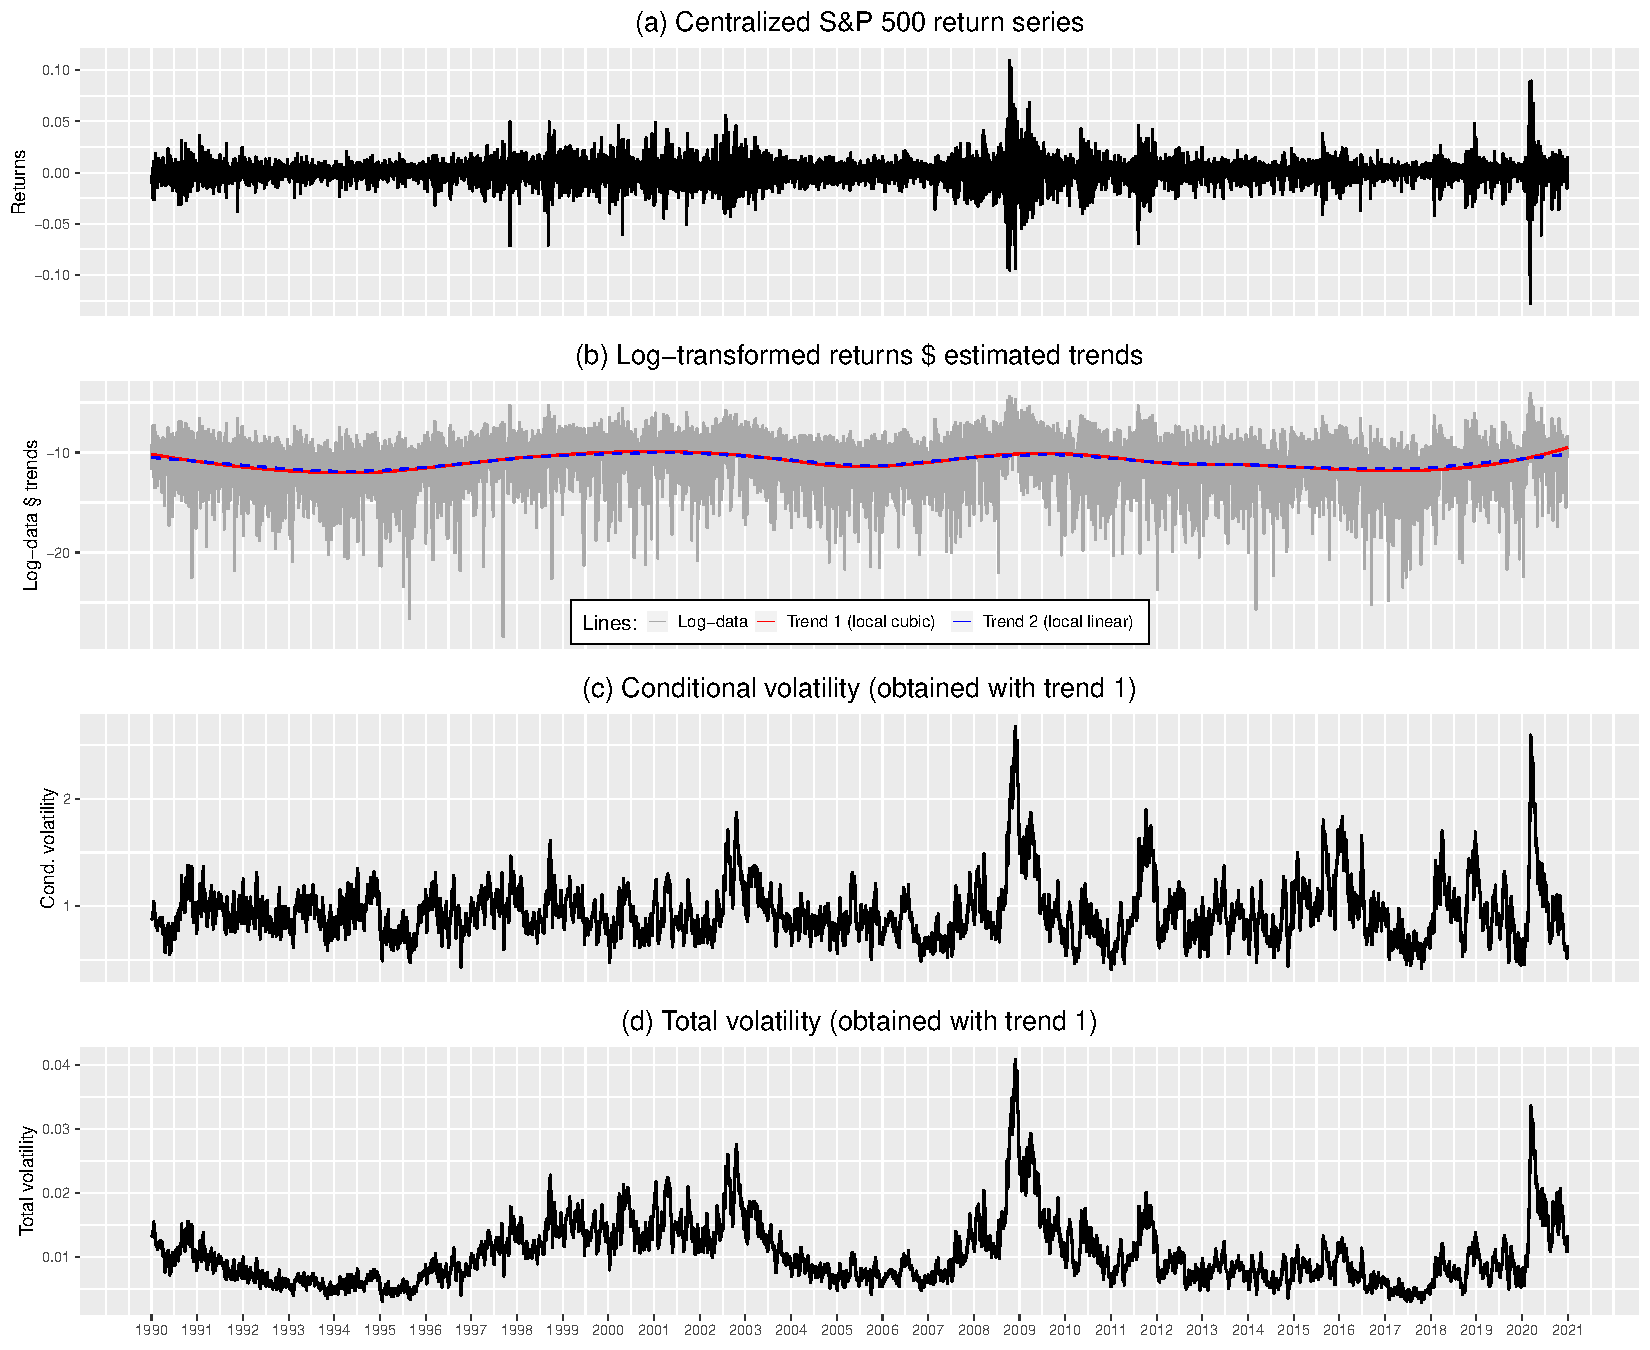
\includegraphics[trim={0mm 0mm 0mm 0mm}, width=\textwidth, height=17cm]{SP500.pdf}		
%\end{figure}
\clearpage
\begin{lstlisting}[language=Python]
> ... test
\end{lstlisting}
PGARCH

Succarat 2016

Francq 2013

\clearpage
\printbibliography
\end{document}
